\section{Method}
    
    \frame{\sectionpage}
    
    \begin{frame}{Adaptive Method}
        \begin{itemize}
            \item 1/5 Success Rule
            \item Average Fitness
            \item Generations
            \item Diversity
            \item Cosine Similarity
            % \item Shannon Entropy
            \item Mating Distance
        \end{itemize}
    \end{frame}

    \begin{frame}{Average Fitness}
        \begin{itemize}
            \item Individual-Based
                \begin{itemize}
                    \item For each individual, if its fitness is lower than the average fitness of the population, increase the mutation rate.
                    \item This encourages exploration for individuals that are not performing well compared to the population.
                \end{itemize}
            \item Global-Based
                \begin{itemize}
                    \item Compare the current average fitness with the previous average fitness of the population.
                    \item If the average fitness stagnates or doesn’t improve, increase mutation rate to reintroduce diversity and avoid local minima.
                    % \item This approach is more global and looks at overall population performance.
                \end{itemize}
        \end{itemize}
    \end{frame}

    \begin{frame}{Generations}
        \begin{itemize}
            \item Adjust the mutation step size according to difference phase of the searching process.
            \item Inspired from the scheduler of gradient descent.
            \item A larger mutation step size is applied at the beginning to increase exploration.
            \item Progressively lower the mutation step size to increase the exploitation.
            \item One typical approach is Cosine Annealing. \cite{loshchilov2017sgdrstochasticgradientdescent}
        \end{itemize}
        \vspace{10pt}
        \begin{equation*}
            \sigma_t = \sigma_{min} + \frac{1}{2}(\sigma_{max} - \sigma_{min}) \left( 1 + \cos{\left( \frac{T_{cur}}{T_{max}}\pi \right)} \right)
        \end{equation*}
    \end{frame}

    \begin{frame}{Diversity - Distance Function}
        \begin{itemize}
            \item Jaccard Distance \cite{jaccard}
                \begin{equation*}
                    d_J(A, B) = \frac{|A \cup B| - |A \cap B|}{|A \cup B|}
                \end{equation*}
            \item Euclidean Distance
                \begin{equation*}
                    d_J(X_i, X_j) = \sqrt{\sum^n_{k=1} (x_{ik} - x_{jk})^2}
                \end{equation*}
            \item Population Diversity 
                \begin{equation*}
                    \textrm{Average Pairwise Distance} = \frac{1}{N(N-1)} \sum_{i \neq j} d(X_i, X_j)
                \end{equation*}
        \end{itemize}
    \end{frame}

    \begin{frame}{Distance - Drawback}
        \begin{itemize}
            \item Unbounded Range
                \begin{itemize}
                    \item The average pairwise distance can grow unbounded, making it difficult to set a fixed threshold for diversity.
                    \item The threshold would need to be problem-specific, and setting a good value is challenging.
                    \item Can be solved by compare the current diversity with previous generations' results to adaptively set thresholds.
                \end{itemize}
            \item Curse of Dimensionality
                \begin{itemize}
                    \item In higher-dimensional spaces, distances become less meaningful as the points become sparsely distributed.
                    \item Reduces the effectiveness of the diversity measure in large search spaces.
                    \item A well-known example is hubness problem in kNN. \cite{hubness}
                \end{itemize}
        \end{itemize}
    \end{frame}

    \begin{frame}{Cosine Similarity}
        \begin{itemize}
            \item bounded Range [0, 1]
                \begin{itemize}
                    \item Unlike Euclidean distance, Cosine Similarity is bounded within the range [0, 1], making it easier to define thresholds for diversity.
                    \item This ensures a consistent scale across different problems and easier interpretation.
                \end{itemize}
            \item Solving the Curse of Dimensionality
                \begin{itemize}
                    \item Since cosine similarity measures the angle between vectors, it is less sensitive to dimensionality and the sparsity of data.
                    \item In high-dimensional spaces, Euclidean distance can become less meaningful, but cosine similarity remains effective.
                \end{itemize}
        \end{itemize}
        \vspace{-5pt}
        \begin{center}
            \begin{equation*}
                \textrm{Cosine Similarity}(X_i, X_j) = \frac{X_i \cdot X_j}{ \|X_i\| \|X_j\| }
            \end{equation*}
            Where $\cdot$ is dot product, and $\| X \|$ is vector norm.
        \end{center}
    \end{frame}

    \begin{frame}{Mating Distance}
        \begin{itemize}
            \item Select parents for crossover only if their genetic distance exceed certain threshold.
            \item Balancing mating distance helps maintain diversity and avoid premature convergence
        \end{itemize}
    \end{frame}
    
    \begin{frame}{Rastrigin Function}
        A non-convex function that contains a lot of local minima. \cite{rastrigin1974systems,Rudolph1990diploma}
        \begin{equation*}
            f(x) = 10n + \sum^n_{i=1}[ x^2_i - 10 \cos{(2\pi x_i)}]
        \end{equation*}
        \centering
        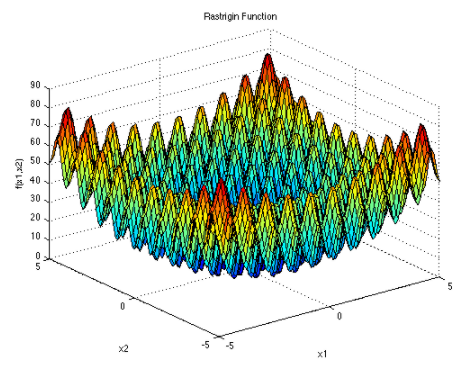
\includegraphics[height = 0.6\textheight]{images/Rastrigin2.png}
    \end{frame}
    
    \begin{frame}{Rosenbrock Function}
    Rosenbrock Function \cite{Rosenbrock} is much smoother than Rastrigin Funciton. \\
    The local minima are in a very narrow valley. \\
    There are two forms of the generalized function. \\
    The first one only defined for even $N$ \cite{Dixon1994-wm}.
    \begin{equation*}
        f(\mathbf{x}) = \sum^{N/2}_{i=1} [100(x^2_{2i - 1} - x_{2i})^2 + (x_{2i-1} - 1)^2]
    \end{equation*}
    The second one is more generalized and contains multiple minima and saddle point \cite{10.5555/534133}:
    \begin{equation*}
        f(\mathbf{x}) = \sum^{N-1}_{i=1} [100(x^2_i - x_ {i+1})^2 + (x_i - 1)^2]
    \end{equation*}

    \end{frame}

    \begin{frame}{Rosenbrock Function}
    \centering
    \colorbox{white}{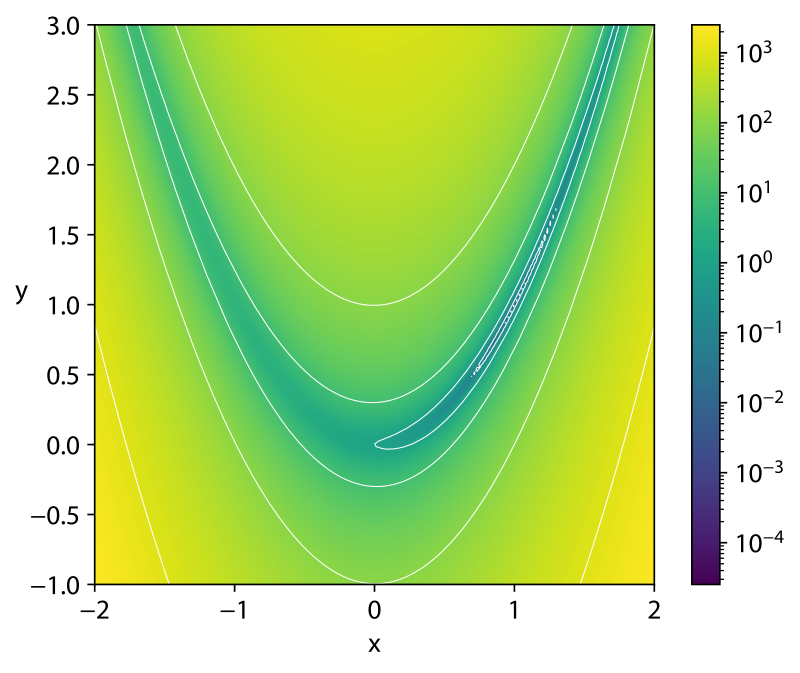
\includegraphics[height=0.7\textheight]{images/Rosenbrock.png}}
    \end{frame}

    \begin{frame}{Sphere Function}
        A smooth convex function.
        \begin{equation*}
            f(x) = \sum^n_{i=1} x^2_i
        \end{equation*}
        \centering
        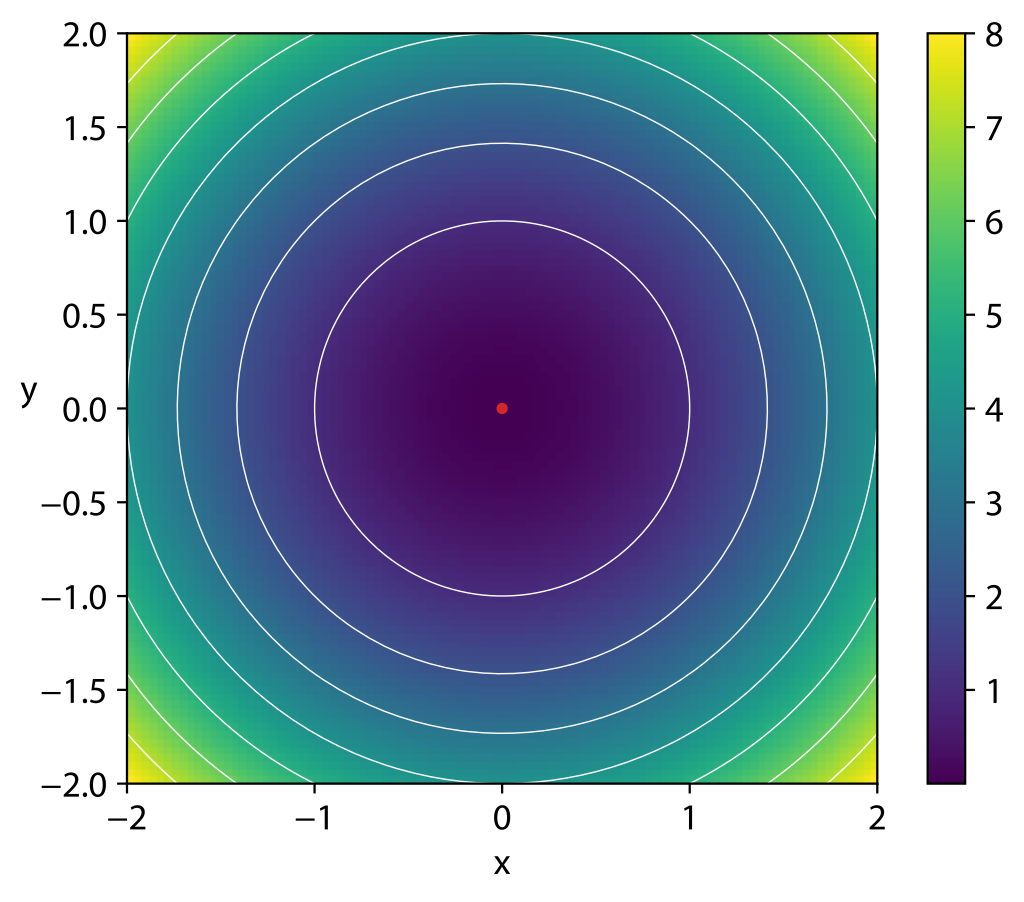
\includegraphics[height=0.6\textheight]{images/Sphere.png}
    \end{frame}

    \begin{frame}{Experiment Setup}
        \begin{itemize}
            \item Population Size: 10
            \item Offspring Size: 50
            \item Parent Selection: Fitness Proportion Selection
            \item Offspring Selection: Elitism without Replacement
            \item Crossover Operator: Discrete Recombination
            \item Mutation Operator: Uniform Mutation
            \item Initial Mutation Step Size: 0.05
            \item Maximum Generation: 100000
            \item Observe Window: 20
            \item Implementation: C++
        \end{itemize}
        More details can be found at \href{https://github.com/isaackhlam/Evolutionary-Computing}{isaackhlam/Evolutionary-Computing}
    \end{frame}
    
